\section{Evaluation}

\begin{changes}

To evaluation our \glspl{name}, we asked two questions.
First, how reliably can automatic explanations could be generated for the expanse of different formats of online tutorials?
Second, can \glspl{exp} help programmers modify existing, unexplained code without having to consult additional documentation?
We answered the first question through collecting a corpus of online tutorials and measuring the detection accuracy of our \glspl{name} for the languages we support.
We address the second question through an in-lab study with programmers modifying unexplained code to perform new tasks, aided by \glspl{name}.

\subsection{Reliability of Snippet Detection}

To determine the reliabilty of our explainable region detection techniques, we first built a corpus of tutorials that used the languages explained by our \glspl{name}.
For each language, we wanted a diversity of tutorials from different domains.
We attempted to achieve diversity of task addressed in the tutorials for the same language by forming queries from common trigrams of StackOverflow tags containing a language.
For example, fetching the most common tags related to CSS selectors yielded several task-specific trigrams including `css-selectors selenium webdriver' (for client-side application testing) and `css-selectors nokigiri ruby' (for web scraping with Ruby).
For each language, for each of the top trigrams from most popular to least used on StackOverflow, we created a Google query by appending the word `tutorial' to the trigram, fetched the first 10 pages from the search results into our corpus, and stopped after we had fetched 300 tutorials.
After one round of filtering we found that 73\% of CSS selector tutorials, 81\% of wget tutorials, and 76\% of regular expression tutorials had at least some code example and was fetched without a download error, yielding >200 tutorials for each language.

We developed a tool to log the locations of manually-selected `ground truth' explainable regions that we found by manually inspecting the tutorials.
Location was stored as a tuple of absolute path to the containing element, and the start and end character indexes of the explainable region within that element.
A match occurred when both the tutoron and a human judge had located an explainable region with exactly the same containing element, and start and end characters.  
`Precision' measured the ratio of correct tutoron detections to the total number of detections, and `recall' measured the ratio of correct tutoron detections to the total number of ground truth explainable regions.

We consistently saw high precision yet low recall with the \glspl{name} (see Table~\ref{tab:detection_accuracy}).    
Low recall can be explained by the fact that code sometimes appears in textual paragraphs, either due to the author's styling preferences, code in unformatted comments at the end of a tutorial, or the author's desire to reference or include a command or abbreviate code snippet in-line with text that describes it.
It is difficult to detect code snippets that are interspersed in textual paragraphs, as there is no textual or structural indicator of where the code starts or ends.
As a result, extra non-code text may be grouped in with the code.
If we restrict \glspl{name} to only scan `code' and `pre' elements on the page, we see an increase in recall to XX-YY\%.
Ultimately, we suspsect that high precision is important to assure \glspl{name} users that the \glspl{exp} illuminate real code, instead of spuriously explaining non-code.
We have yet to verify this experimentally.
While high recall is also important to draw users' attention to explainable code in the browser, \glspl{name} can easily support an architecture where users manually request an explanation for a code snippet that they recognize as being explainable but not automatically detected
\andrew{SIFTER and using machine learning to detect when instances of words are commands.}

\begin{table}
\caption{Accuracy of our explainable region detection.}
\label{tab:detection_accuracy}
\centering
\begin{tabular}{llc}
\toprule
\thead{Language} & \thead{Precision} & \thead{Recall} \\
\midrule
wget & 45\% & 58\% \\ \midrule
CSS selectors & 70\% & 40\% \\ \midrule
RegEx & 41\% & 19\% \\ \bottomrule
\end{tabular}
\end{table}

\subsection{Correctness of Parser}

While our parsers for wget and regular expressions were built on top of existing parsers, we built our simple CSS parser by hand.
We ran our parser against the CSS selectors we extracted from the previous tests as part of our ground truth to see how often it could parse the selectors from the past step without error.
Of the 334 selectors from the last step, 322 (96.4\%) parsed successfully.
Of the 12 that failed to parse, 10 of them could not be lexed as they included incorrectly-formatted characters in the original HTML markup (such as curly quotation marks instead of straight ones) or jQuery-specific pseudo-classes (e.g., \texttt{:jqmData}) that do not belong to the CSS syntax.
With these adjustments, our parser was able to successfully parse 332 our of 334 selectors found online (99.4\%).

\end{changes}

\subsection{In-Lab Usability Study}

We conducted a qualitative usability study to understand how \Glspl{name}-generated \glspl{exp} affected programmers' ability to perform code modification tasks with online example code.
We recruited 9 programmers from university listservs for undergraduate and graduate students in computer science and information science.
All participants had at least two years of programming experience, with a median of 4 years of experience in their longest-used language.  Participants were asked to explain their actions via think-aloud method which was audio-recorded, and their actions were screen-captured and analyzed post-hoc. 

Each participant attempted 8 code modification tasks (plus 2 practice tasks) using two different languages: CSS selectors and \texttt{wget}.
For each language the 4 coding tasks increased in difficulty with the fourth being especially tricky.
We created snippets consisting of a block of code and optionally  explanatory text and comments for each task, based on  existing online programming help.
\begin{changes}
Snippets were from StackOverflow questions or answers.
Tasks asked participants to modify unexplained code from snippets for a purpose unrelated to the StackOverflow question.
\end{changes}
\begin{changes}
While \glspl{name} are designed to help programmers understand code, our tasks focused on code generation and modification.
We see understanding code as central to code modification, and designed tasks to force users to find and understand relevant parts of code.
\end{changes}

Each code modification task consisted of the following steps:
\begin{enumerate}
\item Read a task --- e.g., \emph{write a CSS selector that selects only elements of class \texttt{myInput}.}
\item View a snippet with some clue about the task.
E.g., in Figure~\ref{fig:study_snippet}, the participant was shown a snippet containing CSS selectors that choose elements of class \emph{myCheckbox} without explaining the syntax.
\item Write and test the code in a sandbox we provided.
\end{enumerate}
After reading the snippet, to solve the task, participants could use any resources they wanted to, including searching the web.

\begin{changes}

Example tasks included:
\begin{itemize}

\item
Snippet (excerpt):

\snippet{wget --random-wait -r -p -nd -e robots=off -A``.pdf''  -U mozilla http://math.stanford.edu/undergrad/}

Task: modify the command so it does not automatically fetch the images necessary to display the webpage.

\item
Snippet (excerpt):

\snippet{wget -r -np -N [url] \\}

Task: modify the command to overwrite all files downloaded, even if they have not been updated remotely.

\item

Snippet (excerpt, 1 of 15 lines):

\snippet{\$(`input[id\textasciicircum=``ProductId\_'']')\textbackslash \\  .each(function () \{ }

Task: write a selector that selects only the button elements with IDs starting with bid

\end{itemize}

In one condition, snippets were enhanced with \Glspl{name}.
The \gls{name} did not contain exactly the missing information to complete the task.
For example, for wget tasks, participants were shown descriptions of all options and asked to discover and modify or remove only those relevant to the task.
While these tasks limit the generalizability of our study, we believe that it shows that \Glspl{name} can help in the situations we devised and tested.
\end{changes}

Participants were told they would have 5 minutes for each task; when participants had extra time, if  they had not completed the task, we often asked them to continue so we could observe their problem-solving process. When in the \gls{exp} condition participants were asked to find and view all \glspl{exp} for the source code after reading the snippet.

\begin{figure}
\centering
\framebox{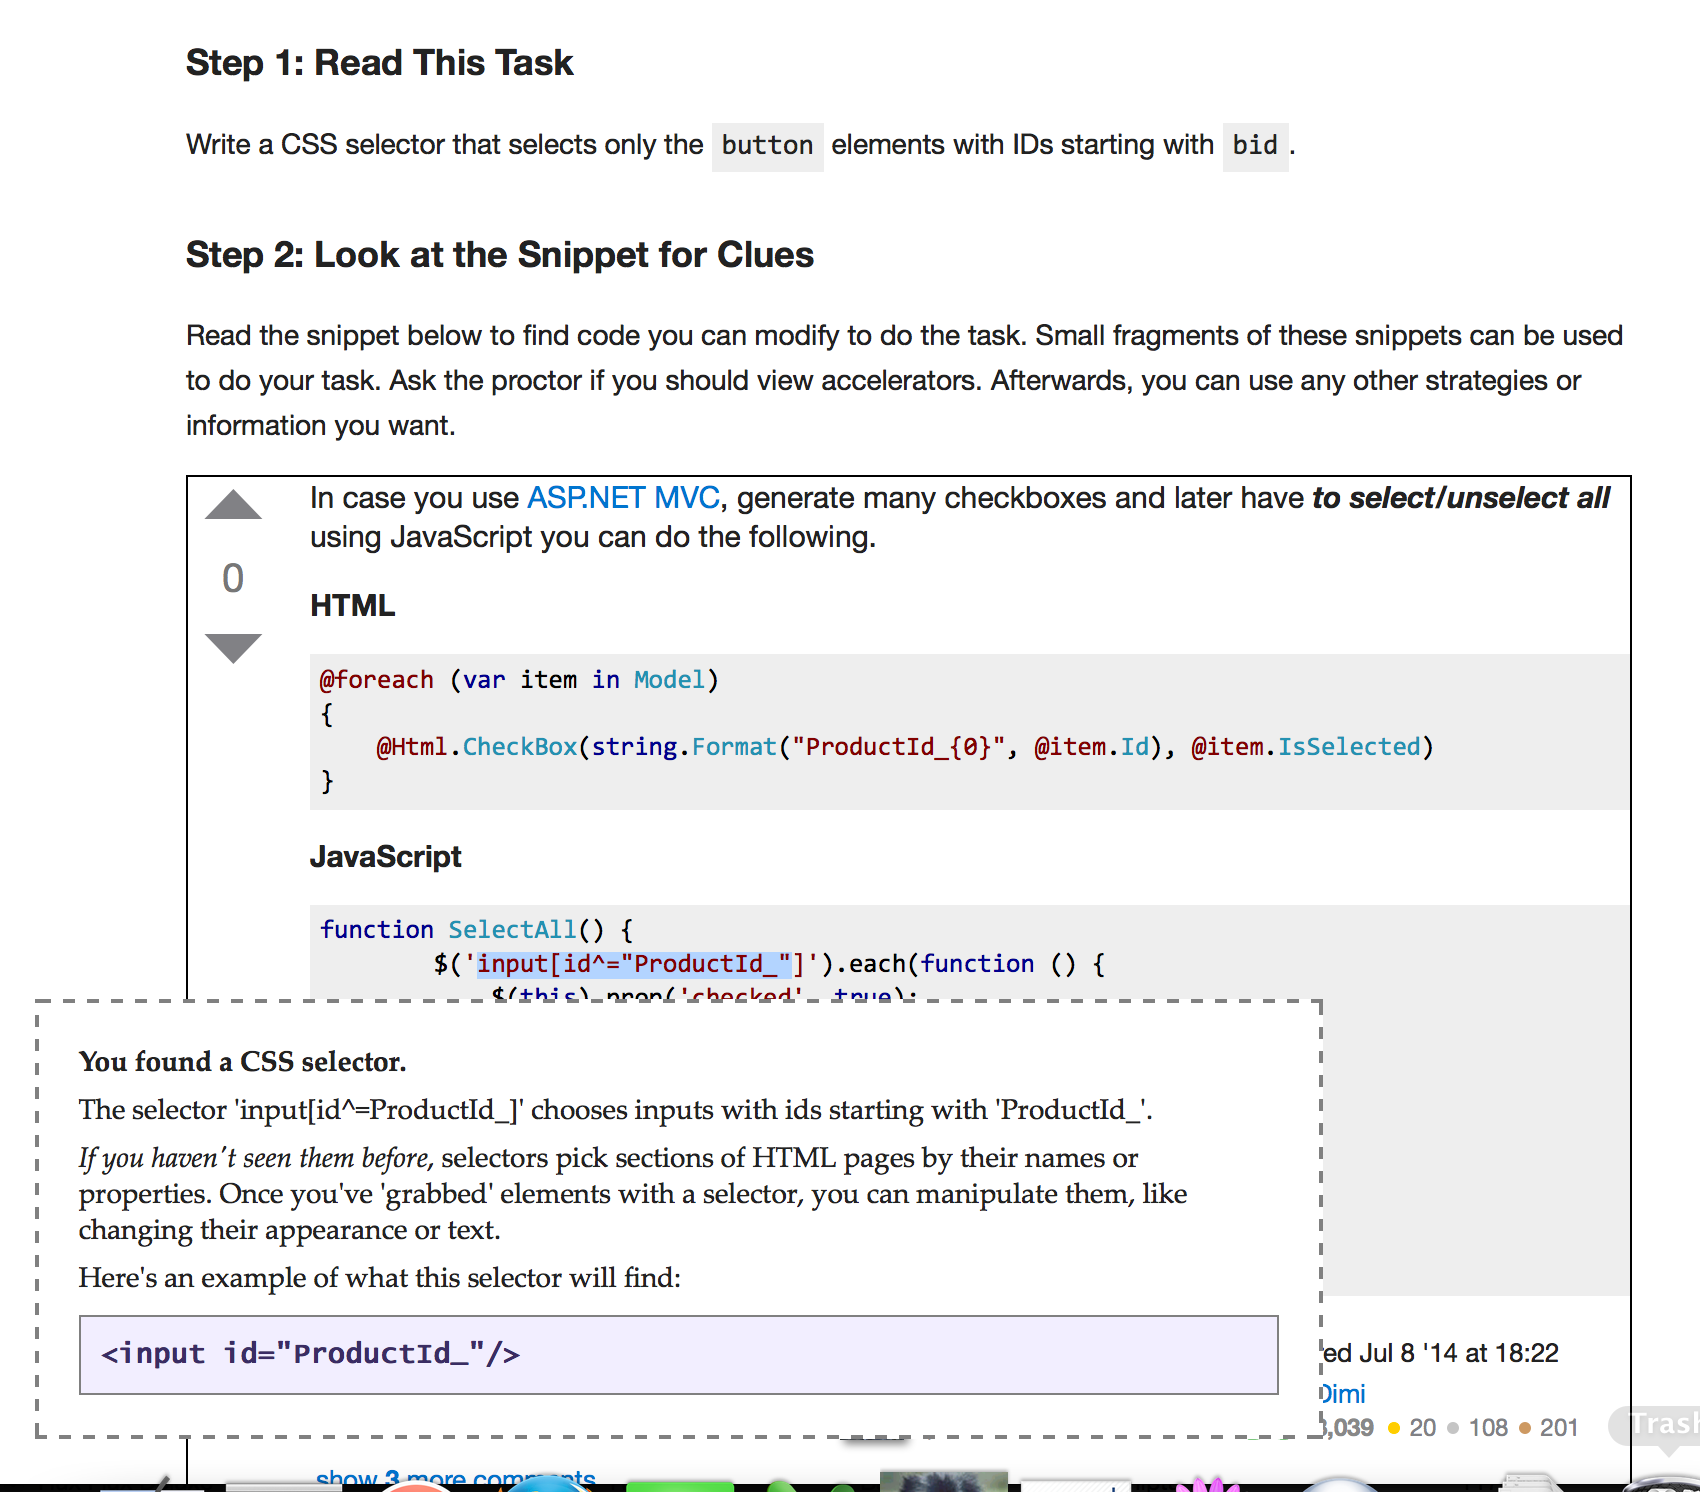
\includegraphics[width=\columnwidth]{figures/study_snippet}}
\caption{An example snippet shown as a clue for a code modification task, accompanied by a \gls{exp} that a participant in our study would have viewed if they were instructed to do so in this task.}
\label{fig:study_snippet}
\end{figure}

Participants viewed \glspl{exp} for alternating tasks so we could observe differences in how they approached the tasks with and without \glspl{exp}; exposure to \glspl{exp} was counter-balanced across participants. 

%%This ordering was counterbalanced across participants so that we could see all tasks performed both with and without \gls{name}-generated \glspl{exp}.

\subsection{Results}

Our primary goal in observing participants was to determine if \gls{name}-generated \glspl{exp} were helpful  during code modification tasks and reduced the need to reference additional documentation.
In the discussion below, we refer to individual participants as $P{1-9}$.

\subsubsection{\Glspl{exp} Help Programmers Modify Code Without Using Other Documentation}

\begin{figure}
\centering
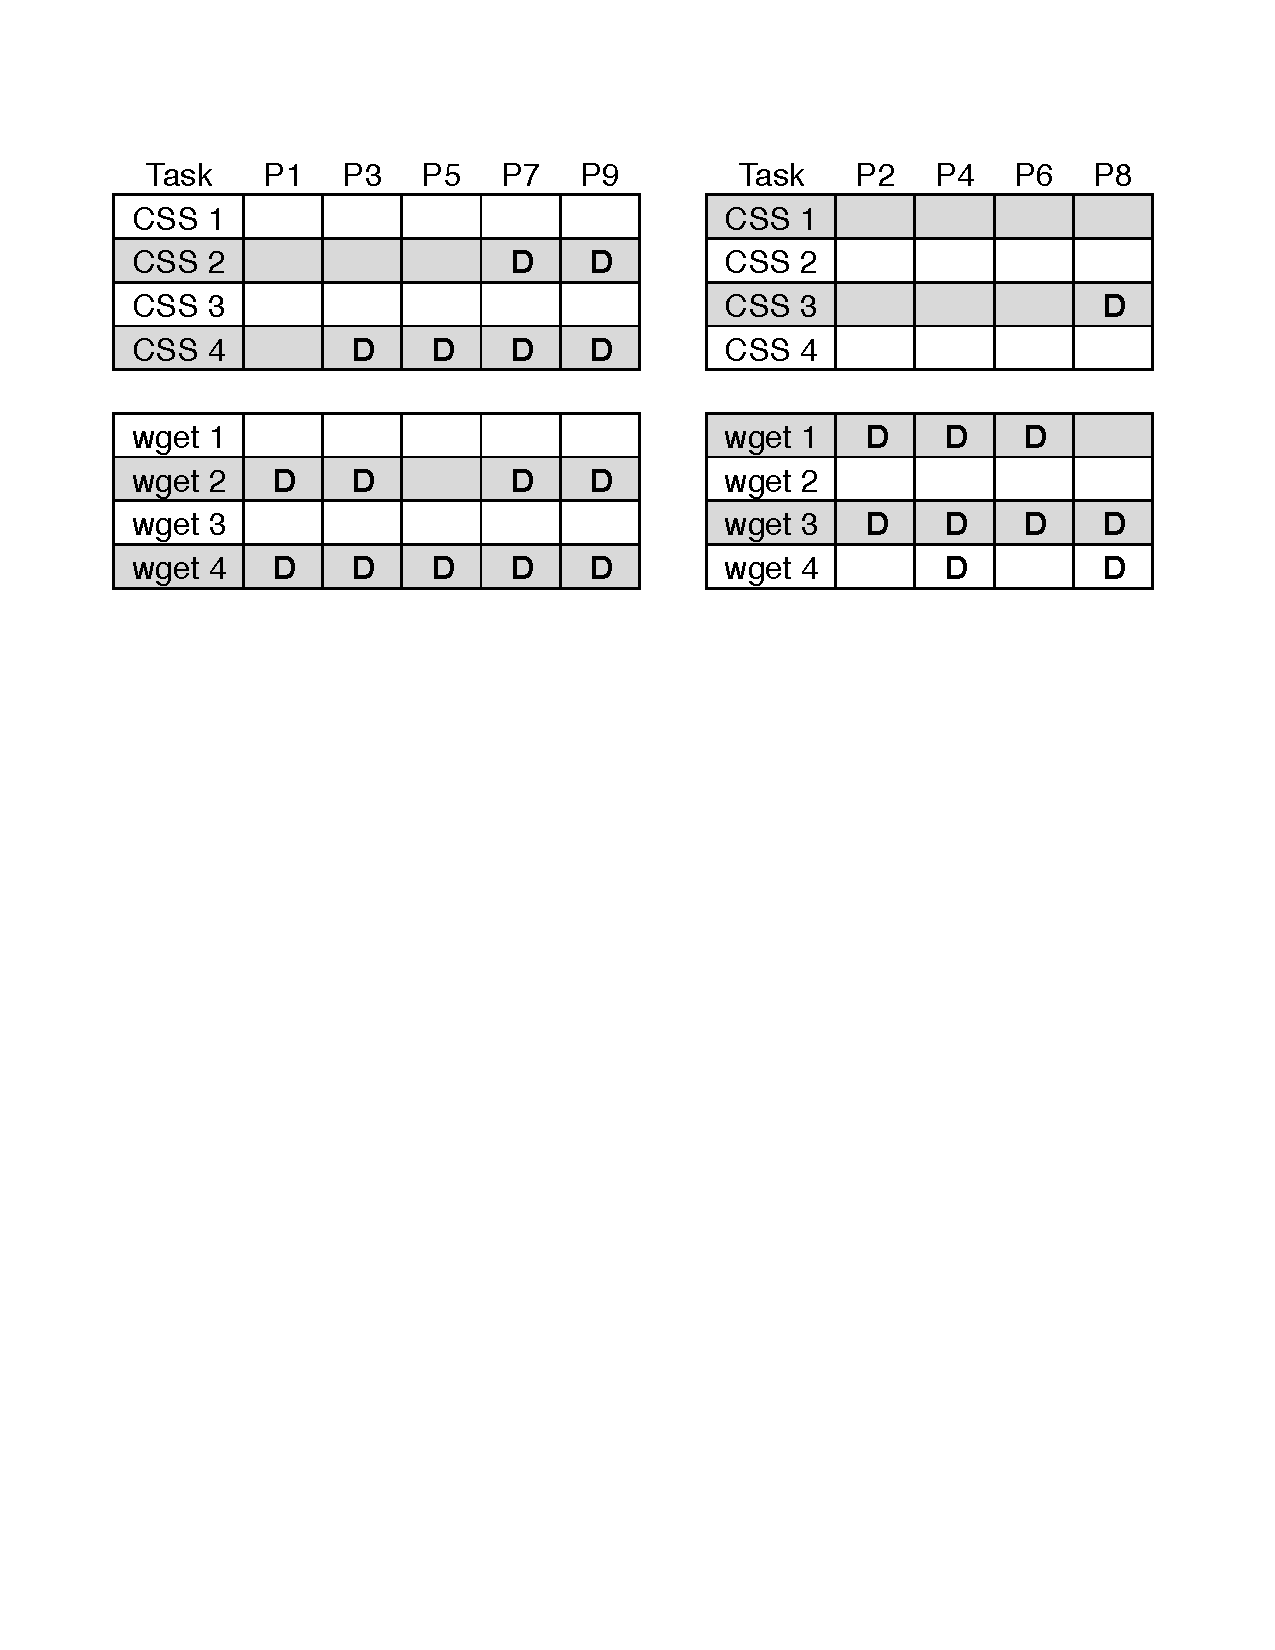
\includegraphics[width=\columnwidth]{figures/doc_accesses}
\caption{%
Tasks for which participants sought additional documentation beyond the snippet. In white rows, participants used \glspl{exp}; in gray rows, they did not.
A cell is marked with the letter `D' if a participant accessed external documentation during that task.
}
\label{fig:doc_accesses}
\end{figure}

When using the \glspl{exp}, 34 out of 36 tasks, or 94\% did not require external documentation.  However, for those tasks where \glspl{exp} were not available, 63\% of the time participants did indeed access external resources in order to complete the task.  The wget tasks especially required external help, with man pages and other resources being accessed in 89\% of cases.  
A detailed breakdown of external document usage is shown in Figure~\ref{fig:doc_accesses}. 


%%In total, out of 72  tasks, participants sought out additional documentation a total of 25 times (Figure~\ref{fig:doc_accesses}).
%%In all wget tasks and in the fourth CSS selector task, a majority of participants without \glspl{name} viewed documentation at some point while trying to find a solution to the problem.
%%In the all 4 CSS selector tasks and the first 3 wget tasks, no participants with access to the \glspl{exp} sought additional documentation in order to solve the problem.

%Only in the final wget task did any participants with access to \glspl{name} seek documentation.


These preliminary results suggest that the \glspl{exp} are effective at reducing the need to switch contexts to find relevant programming help  for completing some programming tasks. 
The \gls{exp} aided the programmers in several ways:

{\bf Reducing need to access external documentation.}
Participants were  able to identify which flags had to be removed from wget commands without consulting external documentation, despite not having used the wget before ($P4$).
For others, the \gls{exp} affirmed a guess that the participant already had about how to construct a CSS selector ($P1$).

{\bf Context-relevant pattern matching.}
One participant noted that the \glspl{exp} helped  to map flags for the wget command line to the higher-level intent of the task ($P4$). 
For the most complex CSS selector task (see Figure~\ref{fig:study_snippet}), two participants noted
that the example HTML shown in the \gls{exp} 
provided a pattern of what fields needed to be changed  from the selector in the snippet to capture the element and ID required by the task prompt ($P2$, $P4$).

{\bf Learning programming concepts.}
For another participant with little previous experience with CSS selectors, a \gls{exp} in  the first task provided him with the knowledge needed to write the selector for the next two tasks, one task for which he was not allowed to view \glspl{exp} ($P5$).

\subsubsection{Programmers Without \Gls{exp} Searched External Documentation}

Some of the difficulties participants faced in the no-\gls{exp} condition  highlight the benefits of in-situ help.
Some participants had difficulty searching for programming help on a web search engine (Google) and using the seach results.
One participant could not express the symbols `\texttt{\^{}=}' as a query term when searching for what  this pattern signifies in CSS selectors.
Her follow-up queries with English language query terms  yielded search results that were not relevant ($P3$).

Participants also had difficulty navigating conventional forms of programming help.
When looking for the \texttt{-r} flag in the man page for wget ($P2$, $P4$), participants found that a page-internal  search for the flag yielded so many matches that it was difficult to find the desired definition.
The description of the \texttt{-N} timestamp flag that was relevant to the code modification task was not directly adjacent to where the flag was introduced, causing one participant to overlook this information, even though it was only 10 lines away ($P3$).

These results underscore the usefulness of context-relevant explanations located within the tutorial text itself.

\subsubsection{Opportunities for Improvement}
In those cases where the \gls{exp} did not aid programmers, there were a few primary causes.

{\bf No visual affordances.} We did not place  visible cues showing where explanations were available.
Programmers may fail to find \glspl{exp} since they have to be explicitly invoked through a right-click.
Although $P2$ eventually found a \gls{exp} that led him to writing a successful CSS selector for the most difficult CSS task, he had to click around the snippet to find it, and did so only upon being reminded by the experimenter that he had not viewed all the \glspl{exp} in the snippet ($P2$).  We plan to experiment with providing visual affordances for the presence of \glspl{exp} in future.


{\bf Selection region ambiguity.}
The leniency of our algorithm for matching a text selection to an explained code fragment caused confusion for programmers about which fragments would be explained on each page ($P1$, $P2$, $P5$).
For the same reason, explanations generated did not always match the fragment selected ($P1$, $P3$, $P5$).
For example, one participant selected the text \texttt{<p>} for which no explanation was generated by the explanation server, because no CSS selector starts with a less-than sign.
However, our selection matching algorithm matched this string to the \texttt{p.mainPageMeters} selector for which an explanation \emph{had} been generated by the server.  As a result, this participant viewed an irrelevant explanation for the code fragment he was viewing ($P5$).  More work is required to determine the right balance of fuzziness for the matching algorithm, with perhaps a drop-down menu of choices for alternative matches.

{\bf Incomplete explanations.} The  \gls{exp} text may not include enough detail to help programmers  develop adequate mental models of unfamiliar material. For instance,
even after completing all 4 CSS selector tasks, $P5$ appeared to believe that CSS selectors were HTML elements themselves, rather than labels that could fetch them, perhaps confused by the example HTML produced in each \gls{exp} ($P5$).  That said, the idea of \gls{exp} can be expanded by adding links to fuller tutorial material.
